\documentclass[11pt,letterpaper]{article}
\usepackage[utf8]{inputenc}
\usepackage[left=1in,right=1in,top=1in,bottom=1in]{geometry}
\usepackage{amsfonts,amsmath}
\usepackage{graphicx,float}
\usepackage{esint}
\usepackage{csquotes}
% -----------------------------------
\usepackage{hyperref}
\hypersetup{%
  colorlinks=true,
  linkcolor=blue,
  citecolor=blue,
  urlcolor=blue,
  linkbordercolor={0 0 1}
}
% -----------------------------------
\usepackage[authordate,backend=biber]{biblatex-chicago}
\addbibresource{citation.bib}
% -----------------------------------
\usepackage{fancyhdr}
\newcommand\course{MATH-UA.0230, PHYS-UA 180\\Introduction to Fluid Dynamics}
\newcommand\hwnumber{5}                  % <-- homework number
\newcommand\NetIDa{Ryan Sh\`iji\'e D\`u} 
\newcommand\NetIDb{March 2nd, 2023}
\pagestyle{fancyplain}
\headheight 35pt
\lhead{\NetIDa\\\NetIDb}
\chead{\textbf{\Large Worksheet \hwnumber}}
\rhead{\course}
\lfoot{}
\cfoot{}
\rfoot{\small\thepage}
\headsep 1.5em
% -----------------------------------
\usepackage{titlesec}
\renewcommand\thesubsection{(\arabic{section}.\alph{subsection})}
\titleformat{\subsection}[runin]
        {\normalfont\bfseries}
        {\thesubsection}% the label and number
        {0.5em}% space between label/number and subsection title
        {}% formatting commands applied just to subsection title
        []% punctuation or other commands following subsection title
% -----------------------------------
\setlength{\parindent}{0.0in}
\setlength{\parskip}{0.1in}
% -----------------------------------
\newcommand{\de}{\mathrm{d}}
\newcommand{\DD}{\mathrm{D}}
\newcommand{\pe}{\partial}
\newcommand{\mcal}{\mathcal}
%\newcommand{\pdx}{\left|\frac{\partial}{\partial_x}\right|}

\newcommand{\dsp}{\displaystyle}

\newcommand{\norm}[1]{\left\Vert #1 \right\Vert}
%\newcommand{\mean}[1]{\left\langle #1 \right\rangle}
\newcommand{\mean}[1]{\overline{#1}}
\newcommand{\inner}[2]{\left\langle #1,#2\right\rangle}

\newcommand{\ve}[1]{\boldsymbol{#1}}

\newcommand{\thus}{\Rightarrow \quad }
\newcommand{\fff}{\iff\quad}
\newcommand{\qdt}[1]{\quad \mbox{#1} \quad}

\renewcommand{\Re}{\mathrm{Re}}
\renewcommand{\Im}{\mathrm{Im}}
\newcommand{\E}{\mathbb{E}}
\newcommand{\lap} {\nabla^2}
\renewcommand{\div}{\nabla\cdot}

\newcommand{\csch}{\text{csch}}
\newcommand{\sech}{\text{sech}}


\newcommand{\hot}{\text{h.o.t.}}

\newcommand{\ssp}{\left.\qquad\right.}

\newcommand{\var}{\text{var}}
\newcommand{\cov}{\text{cov}}


\begin{document}

\section{Energy dissipation in Navier-Stokes}
Remember that the incompressible Navier-Stokes can alternatively be written as
\begin{align}
    \rho\frac{D\ve v}{Dt} &= -\nabla p-\mu\nabla\times\ve \omega.
\end{align}

\subsection{}
Show the vector identity
\begin{align}
    \nabla\cdot(\ve a\times\ve b) = (\nabla\times\ve a)\cdot\ve b-\ve a\cdot(\nabla\times\ve b).
\end{align}

\subsection{}
[From \cite{Aris_62}, Exercise 6.14.4] For an incompressible Newtonian fluid moving within a fixed stationary boundary with no body forces, show that the total rate of dissipation of kinetic energy is
\begin{align}
    -\mu \iiint_V \ve\omega^2 \;\de V.
\end{align}

\subsection{}
To get another form of the total rate of dissipation of kinetic energy, we can work with the dissipation in Navier-Stokes directly. Dot it with $\ve v$ and integrate over the domain, we have
\begin{align}
    \mu \iiint_V \ve v\nabla^2\ve v \;\de V &= -\mu \iiint_V \nabla \ve v:\nabla\ve v \;\de V.
\end{align}

\subsection{}
In lecture you learned the total rate of dissipation of kinetic energy is
\begin{align}
    -2\mu \iiint_V \ve E:\ve E \;\de V.
\end{align}
These three forms should all be equal. Make sense of this by assume 
\begin{align}
    \iiint_V \ve E:\ve E \;\de V = \iiint_V \ve W:\ve W \;\de V.\label{eq:EW_ident}
\end{align}

\subsection{}
Now show
\begin{align}
    \iiint_V \nabla \ve v:\nabla\ve v^\top \;\de V = 0.
\end{align}
Show that this implies \eqref{eq:EW_ident}.

\newpage
\section{Vena contracta}
[From \cite{Falkovich_18}, \S 1.1.4] We have derived the flow speed for the efflux from a small orifice under the action of gravity from Bernoulli's principle. It follows the Torricelli formula $v = \sqrt{2gh}$. We now will derive the rate of discharge. Suppose the opening size on the side-wall is $S$, in reality, the discharge rate will not be $vS$, because of the phenomenon called vena contracta. As a first understanding, I quote the explanation in Falkovich's book:
\begin{displayquote}
    Indeed, streamlines converge from all sides toward the orifice so that the jet continues to converge for a while after coming out (Figure below). Moreover, the converging motion makes the pressure in the interior of the jet somewhat greater than that at the surface (as is clear from the curvature of streamlines) so that the velocity in the interior is somewhat less than $\sqrt{2gh}$. The experiment shows that contraction ceases and the jet becomes cylindrical at a short distance beyond the orifice. This point is called ``vena contracta'' and the ratio of the jet area there to the orifice area is called the coefficient of contraction. The estimate for the discharge rate is $\sqrt{2gh}$ times the orifice area times the coefficient of contraction. For a round hole in a thin wall, the coefficient of contraction is experimentally found to be 0.62.
\end{displayquote}
\begin{figure}[H]
    \centering
    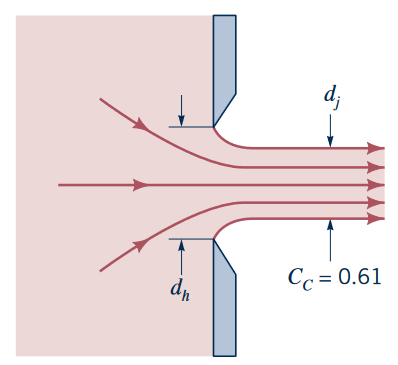
\includegraphics[width=0.5\textwidth]{figs/vena_contracta}
    \caption{Picture from \cite{GerhartEtAl_20}.}
\end{figure}

We will work through a slightly different set-up called Borda mouthpiece where the coefficient of contraction could be obtained by hand. The Borda mouthpiece is a cylindrical tube, projecting inward to the center of the bucket.
\begin{figure}[H]
    \centering
    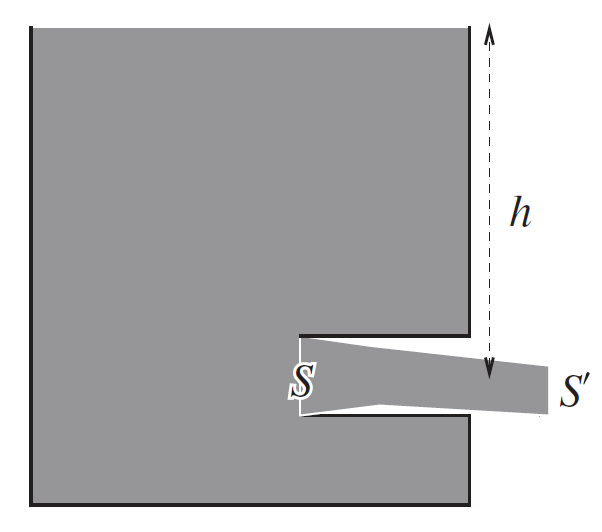
\includegraphics[width=0.4\textwidth]{figs/borda}
\end{figure}
Name $S'$ the size of the jet area so that the coefficient of contraction is $S'/S$. 

\subsection{}
Assume $S'$ given, what is the discharge rate. What is the momentum flux of this discharge.

\subsection{}
We know that the horizontal momentum flux should be equal to a surface integral of the force from the wall of the bucket. Use this relation, and $v=\sqrt{2gh}$ to obtain the coefficient of contraction is $S'/S = 0.5$.

    
\vfill
\printbibliography


\end{document}